\documentclass[11pt,a4paper]{article}
\usepackage[utf8]{inputenc}
\usepackage[french]{babel}
\usepackage[T1]{fontenc}
\usepackage{amsmath}
\usepackage{amsfonts}
\usepackage{amssymb}
\usepackage{soul}
\usepackage{graphicx}
\usepackage[left=2cm,right=2cm,top=2cm,bottom=2cm]{geometry}
\author{Tafsir GNA}
\title{Résolution du "Pigment Sequencing Problem" avec les algorithmes génétiques}
\begin{document}

\hrule
\begin{center}
	\textbf{Rapport 1 de travail du \today{} sur la résolution du "Pigment Sequencing Problem" avec les algorithmes génétiques}
\end{center} 
\hrule

\begin{center}
	\textbf{Tâche à faire :} Implémentation préliminaire d'un algorithme génétique pour la résolution du "Pigment Sequencing Problem" 
\end{center}

\section{Modélisation du problème}
	L'objectif est de trouver un plan de production d'articles sur un horizon de planification discret et fini. Afin d'y parvenir, nous avons décidé d'appliquer une méthode de recherche basée sur les algorithmes génétiques. Les algorithmes génétiques fonctionnent sur une population de individus appelés "chromosomes". Ces derniers représentent une solution admissible aux problèmes. Les algorithmes génétiques font évoluer cette population initiale d'individus à travers différentes itérations appelées "générations". Cette évolution se fait à travers l'application sur une population d'opérateurs génétiques tels que la sélection, la reproduction (crossover), la mutation jusqu'à ce qu'un point de terminaison soit atteint. Afin d'appliquer notre méthode génétique, la représentation suivante a été retenue. \\
	\hspace*{.5cm} Dans le cas, de 2 articles à produire sur une horizon de planification de 5 périodes, le chromosome suivant : [2, 1, 0, 1, 2] avec des demandes pour l'article 1 de [0, 1, 0, 0, 1] et pour l'article 2 de [1, 0, 0, 0, 1]. Dans une autre cas encore de 3 articles sur 8 périodes avec des demandes de [0, 0, 0, 0, 0, 1, 0, 1] pour l'article 2, [0, 0, 1, 1, 0, 0, 1, 0], et [0, 0, 0, 0, 0, 0, 1, 0] pour l'article 3, un chromosome peut être représenté comme suit : [1, 1, 2, 2, 0, 3, 2, 0]. \\
	\hspace*{.5cm} Deux formats de fichiers pour les entrées ont été retenus:\\
	\\
	\hspace*{.5cm} \textbf{\emph{Premier format}:}
	\begin{verbatim}
	Items = 3;

	Demands = [|0, 0, 0, 0, 0, 1, 0, 1
			|0, 0, 1, 1, 0, 0, 1, 0
	   		   |0, 0, 0, 0, 0, 0, 1, 0|];

	StockingCosts = [10, 15, 12];

	SetupCosts = [|0, 131, 109
	      |193, 0, 175
              |101, 136, 0|];
	\end{verbatim}
	
	\textbf{\emph{Deuxième format}:}
	
	\begin{verbatim}
	20
	5
	20

	0 18 21 32 41
	16 0 33 22 17
	38 16 0 21 31
	12 18 44 0 37
	49 41 40 29 0

	19 32 42 32 11

	0 0 0 0 0 0 0 0 0 0 1 1 0 0 0 0 0 0 1 1
	0 0 0 0 1 0 0 1 0 1 0 0 0 0 1 0 0 1 0 1
	0 0 0 0 0 0 0 0 1 0 0 1 0 0 0 1 0 0 0 1
	0 0 0 0 0 0 1 0 0 0 0 0 0 0 0 0 0 0 1 1
	0 0 0 0 0 1 0 1 0 0 1 0 0 0 0 0 0 0 0 0
	\end{verbatim}

\section{Description de l'algorithme}
	Le programme implémenté se compose des fichiers suivantes : \emph{chromosome.py}, \emph{population.py}, \emph{clsp\_ga\_library.py}, \emph{clsp\_ga.py} et \emph{clsp\_main.py}.
	\subsection{Description des fichiers}
	\subsubsection*{chromosome.py}
	Le fichier \emph{chromosome.py} contient la définition de la classe chromosome. Les attributs de la classe chromosome sont : \emph{solution} qui est la suite de articles produits suivant les périodes (ex. [2, 1, 0, 1, 2]), \emph{fitnessValue} qui est la valeur de fitness attribuée au chromosome en fonction de l'attribut \emph{solution}, \emph{itemsRank} qui indique le rang d'un item à une période donnée dans le plan de planification (ex. [1, 1, 0, 2, 2] pour un attribut \emph{solution} de valeur [2, 1, 0, 1, 2], cet attribut me sert principalement pour l'opération génétique de crossover) et enfin l'attribut \emph{hashsolution} qui est en fait une objet de type string équivalent à la valeur de l'attribut \emph{solution}.
	\hspace*{.5cm} Le chromosome peut donc muter. J'ai donc créer deux fonctions: une fonction de mutation usuelle (\emph{mutation}) qui effectue un changement aléatoire de position à des articles choisis ([2, 1, 0, 1, 2] est une mutation de [2, 1, 0, 2, 1]) et une seconde fonction de mutation avancée que j'utilise dans le cas où je tombe dans une optimum local afin de vérifier si je ne peux pas obtenir un chromosome avec une meilleure valeur de fitness. Le choix a été fait d'effectuer une mutation en une seule plutôt que 2 ou plusieurs points. Deux autres fonctions ont été définies: la fonction \emph{isFeasible} afin de vérifier si le chromosome est admissible par rapport aux contraintes, et le fonction \emph{getFeasible} afin que dans le cas où le chromosome n'est pas admissible, je puisse le rendre admissible.
	
	\subsubsection*{population.py} 
	Le fichier \emph{population.py} contient la définition de la classe population. Dans notre cas, une population est un ensemble de chromosomes et correspond à une génération bien déterminée. Les attributs principaux de la classe chromosome sont : l'attribut \emph{chromosomes} qui est une tableau qui contient l'ensemble des chromosomes de la population, l'attribut \emph{NbPopulation} qui indique la taille de la population; l'attribut booléen \emph{lacksdiversity} qui indique si l'algorithme manque de diversité ou est tombé dans un optimal local. Au nombre des opérations que compte notre classe population, il existe la fonction \emph{applyCrossoverto} qui fait reproduire deux chromosomes choisis suivant la sélection du \emph{"Roulette Wheel"} et la fonction de génération aléatoire des chromosomes qui permet de définir la population initiale à partir de laquelle notre programme va démarrer.
	
	\subsubsection*{clsp\_ga\_library.py}
	Ce fichier décrit une bibliothèque de fonctions où de petites classes utilisées tout au long du programme telles que la classe \emph{Instance} qui définit une instance d'un problème à résoudre ou encore la fonction \emph{"readFile"} de lecture des fichiers d'input.
	
	\subsubsection*{clsp\_ga.py}
	Ce fichier décrit les différentes actions de notre algorithme génétique. Il s'agit d'une classe GeneticAlgorithm qui crée la population initiale et fait évoluer la population sur les différentes générations avant enfin d'afficher le résultat de la recherche.
	
	\subsubsection*{clsp\_main.py} 
	Ce fichier contient le programme principal qui se charge d'initialiser les objets de classes présentées plus haut.\\
	
	En résumé, notre algorithme initialise une population de chromosomes de façon aléatoire. De là notre algorithme sectionne les deux chromosomes parents à reproduire suivant la méthode de "Roulette wheel". Il en résulte deux chromosomes fils qui seront en fonction de leur fitness introduits dans le nouvelle population. La mutation choisit aléatoirement une point de rupture qui sera utilisé pour échanger les caractéristiques de chaque parent sélectionné. Tout cela en vaillant à ce que les chromosomes de la prochaine génération soient toujours admissibles. Lorsque le programme tombe sur un optimal local, il vérifie s'il une meilleure solution ne peut être trouvée. Si oui la recherche continue sinon la popualtion de départ est reprise, amputée de l'optimal local trouvé jusqu'au point de terminaison qui est une paramètre l'algorithme.  
	
\section{Tests et Analyse des résultats}
	Afin de tester le programme, il faut disposer de tous les fichiers sus-cités:
	\begin{center}
		\begin{figure}[h]
			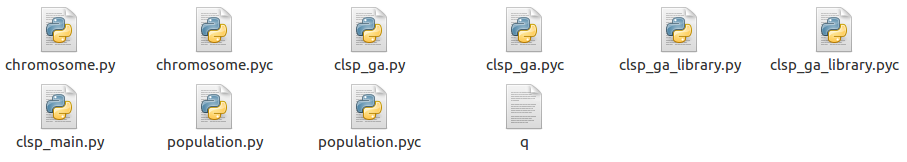
\includegraphics[scale=.5]{img/files.png}
		\end{figure}
	\end{center}
	
	Ouvrir le terminal, se positionner dans le repertoire des fichiers et lancer la commande \emph{./clsp\_main.py} avec le chemin relatif ou absolu du fichier d'input comme le montre l'exemple suivant:
	
	\begin{center}
		\begin{figure}[h]
			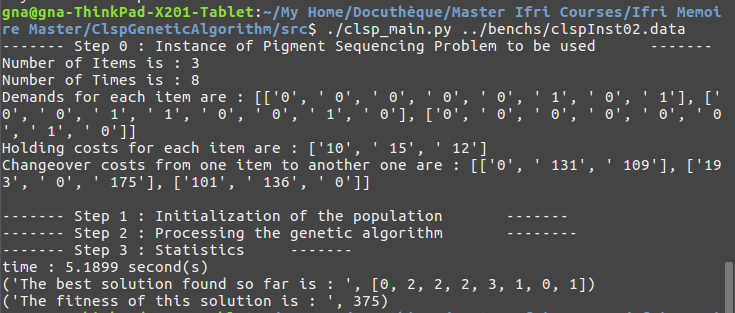
\includegraphics[scale=.5]{img/test.png}
		\end{figure}
	\end{center}
	
	Le programme commence par afficher une donnée de l'instance du problème donné, et après un certain temps de calcul affiché, le programme affiche la solution trouvée et son valeur de fitness.

\end{document}